\thispagestyle{empty}
\topskip0pt
Correlation is an important tool used in Machine Learning for feature extraction on which all the models are based. It involves measuring the relationship between two or more variables in the data set. Quality of the data plays a crucial role in determining the correlations. We will explain different correlations we have identified in the below section.

\subsubsection{Correlations between supply of meeting rooms and demand by employees}
In this section, the supply and demand analysis is carried on meeting rooms and employees.
\begin{enumerate}
    \item If the staff wishes to book a meeting room in the same building where they work, it is observed that building on \textit{333 Exhibition St} has the highest number of meeting rooms(\textbf{29}) and it accommodates only 3\% of the total employee from the data set.
    \item It can be inferred that number of employees located on a particular floor and the corresponding meeting rooms on the floor have a supply-demand problem. For example, \textbf{Doug Mcdonell
} building has 20\% meeting rooms on level 8 out of total meeting rooms in the building for which there is 10\% staff located on that level.
    \item Meeting room usage also depends upon the condition of the room: Out of total meeting rooms across the parkville campus, 81\% of them are in \textit{excellent} condition while 2\% are in very-good condition, 1\% poor and 17\% good.
    \item Meeting room usage and booking can be related to the usage of the meeting room and if they are located at a longer distance from the employee location. \textbf{Stop 1} has the most number of excellent rooms based on the usage data and out of all the meeting rooms, only 3\% can be booked. Buildings with low demand have low usage of the meeting rooms as shown in Figure \ref{usagedata}.

\begin{figure}[H]
    \centering
    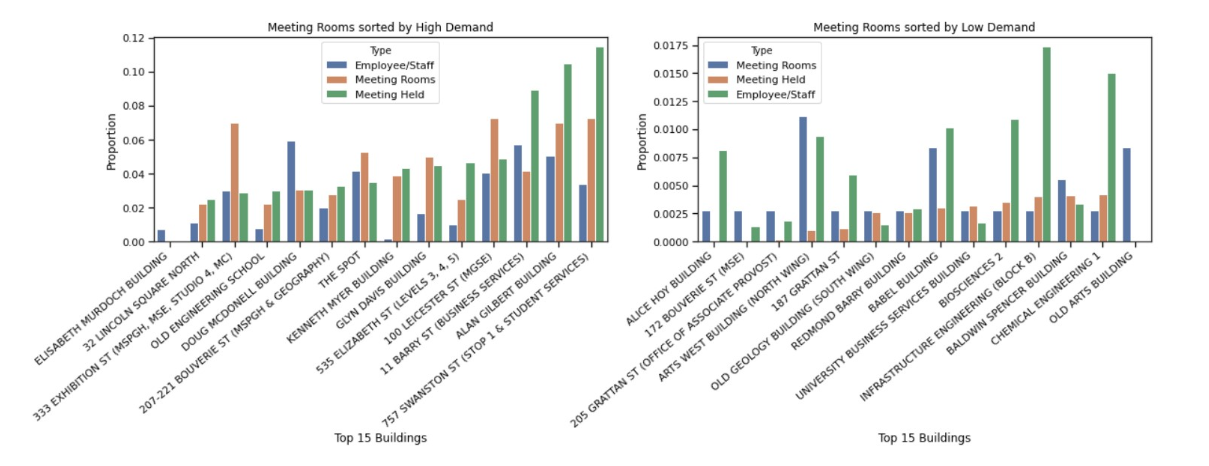
\includegraphics[width=1\textwidth]{resources/images/snap5.PNG}
    \caption{Supply vs demand analysis with meeting room usage correlation}
    \label{usagedata}
\end{figure}

\end{enumerate}

Few correlations are not that strong and can be mentioned as part of the findings of the correlation between data sets. Average attendance, capacity of the meeting room, time of the meeting and the attendance of the meeting are some of the other factors for correlation analysis. An employee would like to book a room with better equipment to enhance the experience.

\subsubsection{Correlations between supply of toilet facilities and demand by students}

In this section, we explore different preferences and factors that correlates with the problem of supply-demand analysis for the toilet facilities.

\begin{enumerate}
    \item Students usually prefer accessing the toilet facilities which are in good condition and in the same building where their respective classes are conducted. We can observe this correlation with respect to supply demand as shown in Figure \ref{toilet}. It can be seen that \textbf{Redmond Barry} has the most number of classes with 8\% of total student and it has mere 2\% of the total excellent toilet capacity to hold possible students. In contrast, Law building has approximately 12\% of the total toilet capacity and around 3\% of total students are attending classes in that building.
    
    \begin{figure}[H]
    \centering
    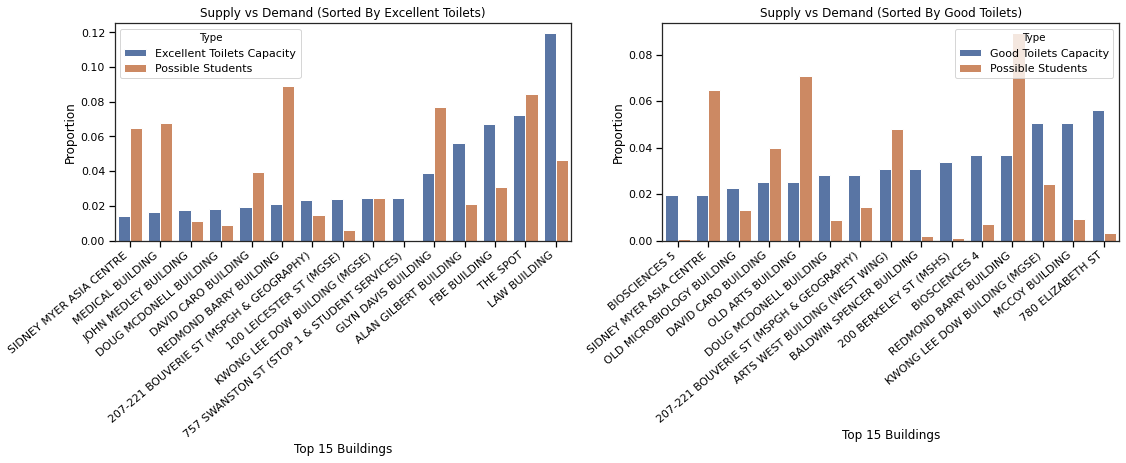
\includegraphics[width=15cm]{resources/images/snap-10.png}
    \caption{Supply vs demand analysis with toilet conditions correlation}
    \label{toilet}
\end{figure}

    \item Students prefer to use the washrooms on the same floor where the lecture hall is situated. Considering Medical Building, it is observed that 30\% of the toilet capacity is available on level 1 while only 5\% of students have lectures on the same floor.
    
    % \item Similarly, based on the toilet condition, students can choose to use the facilities. It is inferred that most of the well-maintained washrooms are in Law building while 4\% students have classes in the same building. The distribution of the condition of facilities is shown in Figure \ref{toilet}.
    
    \item Students can decide to avail the facilities based on the size of the washroom. It is evident that Law building has 5\% of total students and the size of the facilities are not enough with respect to the demand. In contrast, Arts West building has larger toilet facility sizes as compared to the student demand proportion(4.5\%).
    
    \item Duration of classes is also an important correlation to consider in terms of supply and demand of toilet facilities. If classes have longer duration in a building, then that building should have facilities with better capacity. As per our analysis, it can be seen that Old Physics building has very long duration of lectures but it has 1\% of the total capacity of toilets.
    
\end{enumerate}
